\clearpage
\myparagraph{\olly}

Since this example is tricky, let's trace it in \olly.

\olly can detect such switch() constructs, and it can add some useful comments.
\EAX is 2 in the beginning, that's the function's input value: 

\begin{figure}[H]
\centering
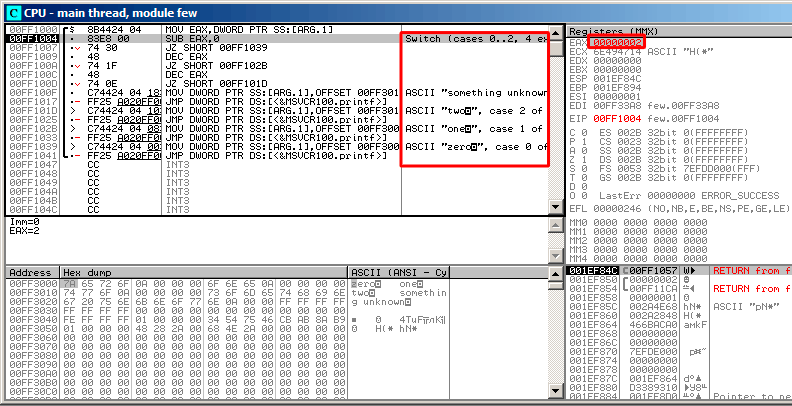
\includegraphics[scale=\FigScale]{patterns/08_switch/1_few/olly1.png}
\caption{\olly: \EAX 
now contain the first (and only) function argument}
\label{fig:switch_few_olly1}
\end{figure}

\clearpage
0 is subtracted from 2 in \EAX. 
Of course, \EAX still contains 2.
But the \ZF flag is now 0, indicating that the resulting value is non-zero:

\begin{figure}[H]
\centering
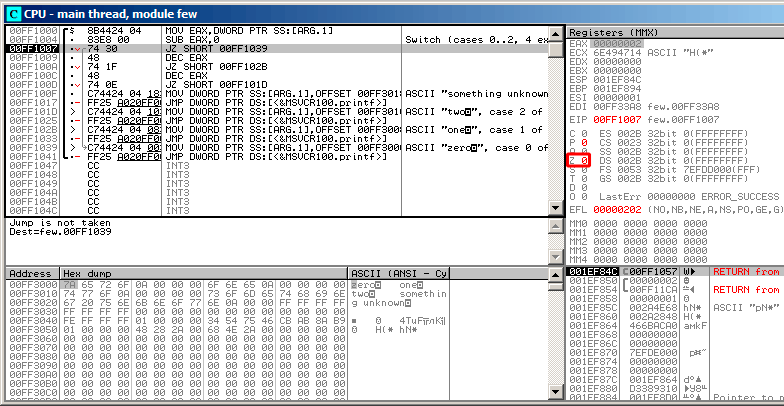
\includegraphics[scale=\FigScale]{patterns/08_switch/1_few/olly2.png}
\caption{\olly: \SUB executed}
\label{fig:switch_few_olly2}
\end{figure}

\clearpage
\DEC is executed and \EAX now contains 1. 
But 1 is non-zero, so the \ZF flag is still 0:

\begin{figure}[H]
\centering
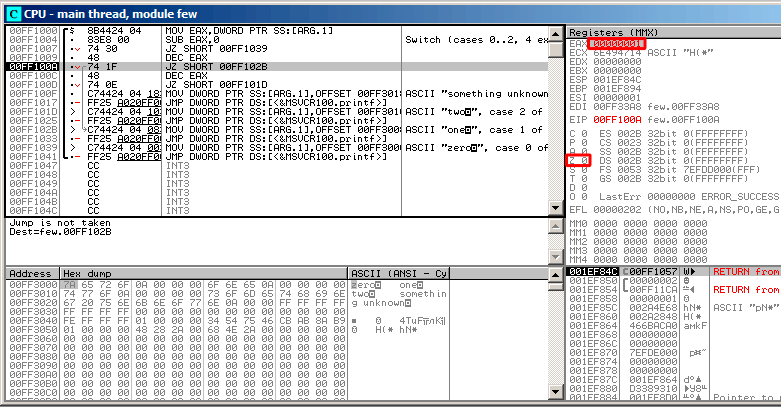
\includegraphics[scale=\FigScale]{patterns/08_switch/1_few/olly3.png}
\caption{\olly: first \DEC executed}
\label{fig:switch_few_olly3}
\end{figure}

\clearpage
Next \DEC is executed. 
\EAX is finally 0 and the \ZF flag gets set, because the result is zero:

\begin{figure}[H]
\centering
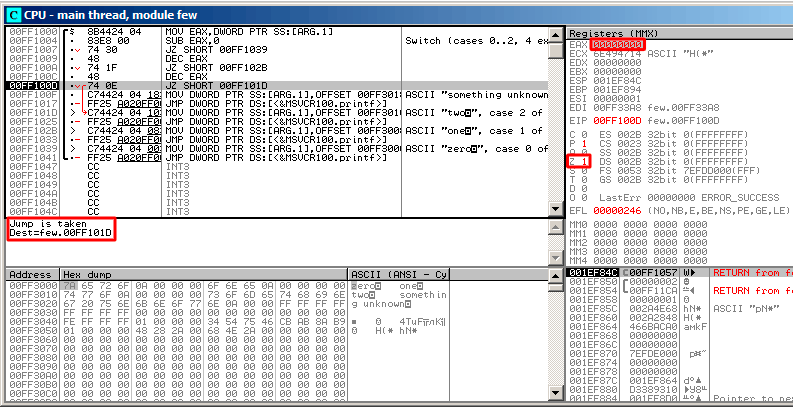
\includegraphics[scale=\FigScale]{patterns/08_switch/1_few/olly4.png}
\caption{\olly: second \DEC executed}
\label{fig:switch_few_olly4}
\end{figure}

\olly shows that this jump is to be taken now.

\clearpage
A pointer to the string \q{two} is to be written into the stack now:

\begin{figure}[H]
\centering
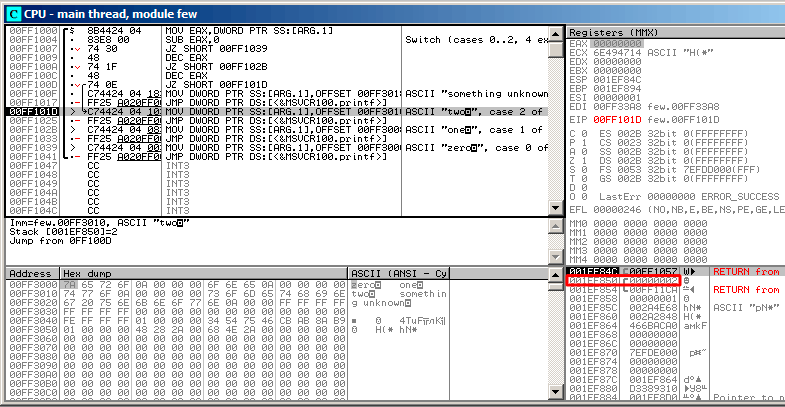
\includegraphics[scale=\FigScale]{patterns/08_switch/1_few/olly5.png}
\caption{\olly: 
pointer to the string is to be written at the place of the first argument}
\label{fig:switch_few_olly5}
\end{figure}

% TODO: homogenize numbers
% now they are inconsistent: sometimes plain text, sometimes in math mode
% some kind of \expr{} both for numbers and expressions? --DY
Please note: the current argument of the function is 2 and 2 is now in the stack at the address \TT{0x001EF850}.

\clearpage
\MOV writes the pointer to the string at address \TT{0x001EF850} (see the stack window).
Then, jump happens.
This is the first instruction of the \printf function in MSVCR100.DLL (This example was compiled with /MD switch): 

\begin{figure}[H]
\centering
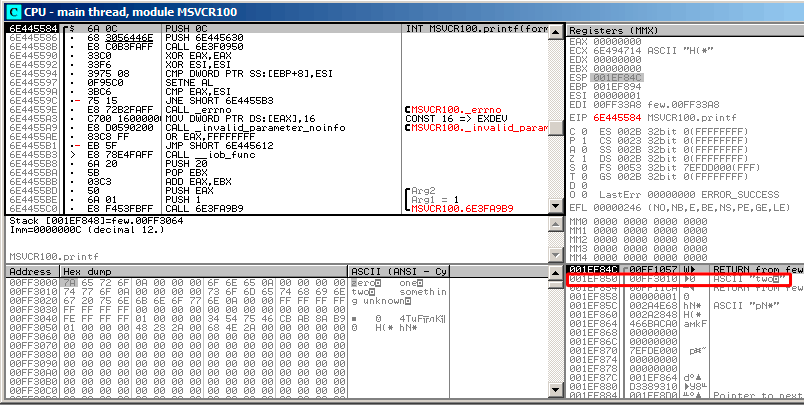
\includegraphics[scale=\FigScale]{patterns/08_switch/1_few/olly6.png}
\caption{\olly: first instruction of \printf \InENRU MSVCR100.DLL}
\label{fig:switch_few_olly6}
\end{figure}

Now \printf treats the string at \TT{0x00FF3010} as its only argument and prints the string.

\clearpage
This is the last instruction of \printf:

\begin{figure}[H]
\centering
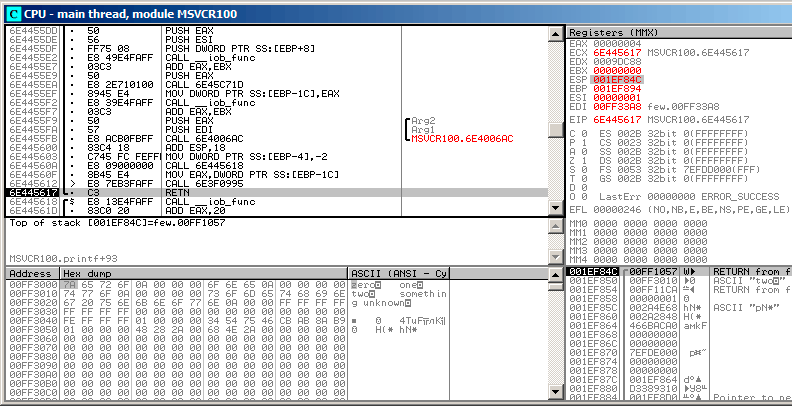
\includegraphics[scale=\FigScale]{patterns/08_switch/1_few/olly7.png}
\caption{\olly: last instruction of \printf in MSVCR100.DLL}
\label{fig:switch_few_olly7}
\end{figure}

The string \q{two} was just printed to the console window.

\clearpage
Now let's press F7 or F8 (\stepover) and return\dots not to \ttf , but rather to \main:

\begin{figure}[H]
\centering
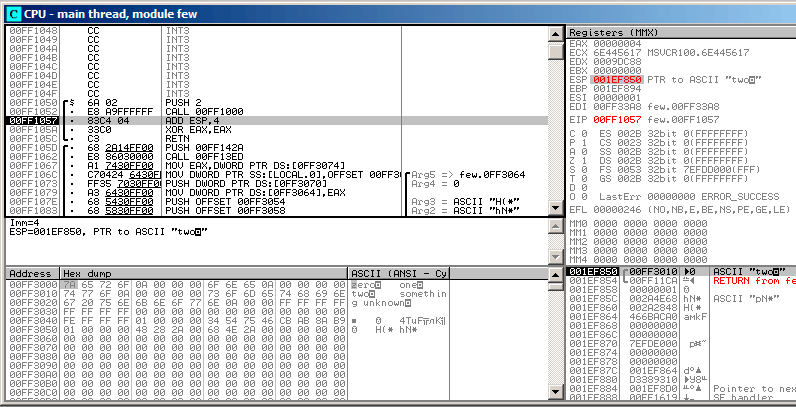
\includegraphics[scale=\FigScale]{patterns/08_switch/1_few/olly8.png}
\caption{\olly: return to \main}
\label{fig:switch_few_olly8}
\end{figure}

Yes, the jump was direct, from the guts of \printf to \main.
Because \ac{RA} in the stack points not to some place in \ttf , but rather to \main.
And \CALL \TT{0x00FF1000} was the actual instruction which called \ttf.

